% THIS IS SIGPROC-SP.TEX - VERSION 3.1
% WORKS WITH V3.2SP OF ACM_PROC_ARTICLE-SP.CLS
% APRIL 2009
%
% It is an example file showing how to use the 'acm_proc_article-sp.cls' V3.2SP
% LaTeX2e document class file for Conference Proceedings submissions.
% ----------------------------------------------------------------------------------------------------------------
% This .tex file (and associated .cls V3.2SP) *DOES NOT* produce:
%       1) The Permission Statement
%       2) The Conference (location) Info information
%       3) The Copyright Line with ACM data
%       4) Page numbering
% ---------------------------------------------------------------------------------------------------------------
% It is an example which *does* use the .bib file (from which the .bbl file
% is produced).
% REMEMBER HOWEVER: After having produced the .bbl file,
% and prior to final submission,
% you need to 'insert'  your .bbl file into your source .tex file so as to provide
% ONE 'self-contained' source file.
%
% Questions regarding SIGS should be sent to
% Adrienne Griscti ---> griscti@acm.org
%
% Questions/suggestions regarding the guidelines, .tex and .cls files, etc. to
% Gerald Murray ---> murray@hq.acm.org
%
% For tracking purposes - this is V3.1SP - APRIL 2009

\documentclass{acm_proc_article-sp}

\usepackage{amsmath}
\usepackage[margin=0.5cm]{caption}
\usepackage{float}
\usepackage{graphicx} % support the \includegraphics command and options
% for osx:
\usepackage[backend=biber]{biblatex}
%\usepackage{biblatex}
\usepackage{subfig}
%\usepackage{subcaption}

\renewcommand{\bibfont}{\footnotesize}
%\pagenumbering{gobble}
\usepackage{hyperref}
\usepackage{booktabs}
\usepackage{multirow}
\usepackage{wrapfig}

\addbibresource{report.bib}


\begin{document}

\title{Parallelised Pose Estimation for Automated Landing}
\subtitle{CS267: Project Report}
%
% You need the command \numberofauthors to handle the 'placement
% and alignment' of the authors beneath the title.
%
% For aesthetic reasons, we recommend 'three authors at a time'
% i.e. three 'name/affiliation blocks' be placed beneath the title.
%
% NOTE: You are NOT restricted in how many 'rows' of
% "name/affiliations" may appear. We just ask that you restrict
% the number of 'columns' to three.
%
% Because of the available 'opening page real-estate'
% we ask you to refrain from putting more than six authors
% (two rows with three columns) beneath the article title.
% More than six makes the first-page appear very cluttered indeed.
%
% Use the \alignauthor commands to handle the names
% and affiliations for an 'aesthetic maximum' of six authors.
% Add names, affiliations, addresses for
% the seventh etc. author(s) as the argument for the
% \additionalauthors command.
% These 'additional authors' will be output/set for you
% without further effort on your part as the last section in
% the body of your article BEFORE References or any Appendices.

\numberofauthors{3} %  in this sample file, there are a *total*
% of EIGHT authors. SIX appear on the 'first-page' (for formatting
% reasons) and the remaining two appear in the \additionalauthors section.
%
\author{
% You can go ahead and credit any number of authors here,
% e.g. one 'row of three' or two rows (consisting of one row of three
% and a second row of one, two or three).
%
% The command \alignauthor (no curly braces needed) should
% precede each author name, affiliation/snail-mail address and
% e-mail address. Additionally, tag each line of
% affiliation/address with \affaddr, and tag the
% e-mail address with \email.
%
% 1st. author
\alignauthor
Sunil Shah\\
       \email{sunil.shah@berkeley.edu}
% 2nd. author
\alignauthor
Nahush Bhanage\\
       \email{nahush@berkeley.edu}
% 3rd. author
\alignauthor 
Hoang Nguyen\\
       \email{hoanghw@berkeley.edu}
}

\date{12 May 2014}

\maketitle
\begin{abstract}
Current approaches for automated landing of unmanned aerial systems (UAS) are
based on GPS localization, which we show is quite inaccurate. We optimise a previously implemented computer vision based pose estimation algorithm to run in real time on a low cost open source embedded computer using open source software. \end{abstract}

%%%%%%%%%%%%%%%%%%%%%%%%%%%%%%%%%%%%%%%%%%%%%%%%%%%%%%%%%%%%%%%%%%%%%%%%%%%%%%
\section{Introduction}
The rise of the hobbyist unmanned aerial system movement has been driven by three factors: 1) the increasing availability and popularity of open source hardware and software, 2) the maker movement and 3) the availability of low cost sensors. These have led to communities such as DIYDrones, a message board where users developed the open source ArduPilot autopilot, initially based on the Arduino platform. In combination with such an autopilot, a user could feasibly 3D print (or purchase) their own multi-rotor frame, mount motors and wire to the autopilot radio control equipment used for ordinary radio control aircraft. For a total cost of approximately \$1,000, a user would have a fully autonomous aerial system.

 As the hobbyist UAS become more capable, an increasing number of researchers and startups are building products and systems using them.  Based on this trend, a federal mandate set in place in 2012 a requirement for the FAA to integrate unmanned aerial systems (UAS) into the national airspace by 2015 for civilian and commercial use.

General purpose open source hardware boards such as the Raspberry Pi or BeagleBone Black typically use the ARM processor architecture, a reduced instruction set computing (RISC) design. This is the architecture most commonly used in smartphones and allows users to run full Linux based operating system such as Ubuntu or Android onboard, with use of with standard libraries and utilities. (This is unlikely prototyping boards such as the Arduino which have their own special purpose environment which is user friendly but limited.) 

While increasing in computing power rapidly, RISC architectures lack the raw performance of more mature and advanced x86 processors which have the same or higher clock speeds but considerably more provisions for fast floating point operations, larger caches and increased processor level parallelism. However, the power, thermal efficiency and spatial gains from using a RISC architecture have made them compelling for power and payload constrained UAS.

In this project, we take a vision based pose estimation algorithm developed for a separate project and investigate parallel processing techniques to optimise its performance on a general purpose open source computer. Current methods of localisation for UAS rely upon GPS, which, unless augmented by additional ground stations transmitting from a known reference location, is inaccurate. In a test run of 10 automated landings where the UAS took off and attempted to land in the same location using GPS, we gained a mean accuracy of 195.33 cm \cite{berzanaccurate}.

Using a landing pad with a known design coupled with a webcam and computer on-board, it is possible to compute considerably accurate pose estimates using computer vision techniques \cite{berzanaccurate}. These permit the UAS to localise itself much more precisely than using GPS alone which enables precision hovering and landing. However, these computer vision techniques are computationally intensive, relying upon several passes over an image to extract features. In our earlier work, we were unable to get this operating at more than 3 frames a second on the BeagleBone Black embedded computer. 

The inner control loop of the ArduPilot autopilot software runs at 10 Hz - where it receives sensor data and outputs a control signal. This is deemed adequate for precise control of a UAS in all but the most extreme environmental conditions. Therefore, for pose estimation to be useful for UAS control, it is necessary to generate pose estimates at a rate of 10 Hz (or, 10 frames per second). Given that, in reality, certain frames are dropped due to motion blur, we strive for a rate of greater than 10 Hz.

We first survey prior work in section \ref{sec:prior-work}, then describe our system architecture in section \ref{sec:system-description}. In section \ref{sec:approach} we detail our approach to optimisation and in section \ref{sec:results} we show the results of this approach.

%%%%%%%%%%%%%%%%%%%%%%%%%%%%%%%%%%%%%%%%%%%%%%%%%%%%%%%%%%%%%%%%%%%%%%%%%%%%%%
\section{Prior Work\label{sec:prior-work}}
Our naive implementation was the result of a previous project and a full description of prior work related to automated landing approaches are available in that paper \cite{berzanaccurate}. The algorithm implemented is described by Sharp et al. in \cite{sharp_et_al_2001} and the overall approach is the same, although the exact implementation details may vary slightly. In their implementation, using highly optimised custom C code, they were able to reach a frame rate of 30 frames per second. 

We consider other prior work related to high performance embedded computing. Several efforts have bene made to explore the effect of parallelising certain robotics appliations but these assume use of a desktop computer and often make use of general purpose computing on the GPU frameworks like CUDA or OpenCL. This doesn't translate well to embedded computers due to the lack of vendor support for graphics chips that are provided. These chips often don't support heterogenous parallel programming languages, such as OpenCL or NVidia's CUDA. 

However, there are several efforts looking at optimising performance for ARM-based processors \cite{mitra2013use}. This is driven by growing smartphone usage, nearly all of which use ARM processor designs. Qualcomm, in particular, provides an ARM-optimised computer vision library for Android called FastCV. While this is optimised for their own series of processors, it does have generic ARM optimisations that are manufacturer agnostic. Efforts have been made to explore OpenCV optimisation for real-time computer vision applications too \cite{pulli2012real}.

A San Francisco based startup, Skycatch Inc., uses a BeagleBone Black to provide a custom runtime environment. This allows their users to write applications on top of their custom designed UAS in scripting language JavaScript. While the user friendliness of this approach is evident, it is also clear that using a high level interpreted application results in a tremendous loss of performance which makes it impossible to do all but the most basic of image processing in real-time. This implementation is also closed source. 

Other commercial entities, such as Cloud Cap Technologies, provide proprietary embedded computers running highly customised computer vision software. However, these cost many thousands of dollars and are difficult to \textit{hack}, making them impractical for research and startup use.

Ultimately, this project's contribution is to demonstrate the tools and techniques that can be used to implement highly performant vision algorithms onboard a UAS using low-cost open source hardware and open source software.

%%%%%%%%%%%%%%%%%%%%%%%%%%%%%%%%%%%%%%%%%%%%%%%%%%%%%%%%%%%%%%%%%%%%%%%%%%%%%%
\section{System Description\label{sec:system-description}}
The intention with this project was to re-use readily available hardware and software as much as possible. Along those lines, we made the decision to use several open source libraries and, as previously mentioned, two open source embedded computers. 

While specific implementation details may only be covered briefly in this paper, detailed instructions, notes and the full source code is available online under the GNU Lesser General Public License at \url{https://github.com/ssk2/drones-267}.

\subsection{Hardware Architecture}

Our overall system architecture is shown in figure \ref{fig:hardware-arch}.

\subsubsection{Autopilot}
Testing was carried out with version 2.6 of 3DRobotics' APM autopilot. This runs their open source ArduCopter autopilot software for VTOL UAS. A full specification is available online \cite{arducopter}. Using a USB cable, we are able to exact high level control of the aircraft using the MAVLink protocol, described further in section \ref{sec:roscopter}.

\subsubsection{Embedded Computer}
Our vision system was implemented on two popular open hardware boards which are both community designed and supported. Documentation is freely available and the boards themselves are produced by non-profit entities. 

We considered boards that could run the entire Linux operating system - for ease of setup and flexibility in software installation. This immediately discounted the archetypical ``Arduino" family of boards - since these are not general purpose computers and cannot run a full installation of Linux. The alternatives are primarily ARM processor based boards - for their low cost processors which have efficient power utilisation \cite{roberts2009arm}.

Our first choice was the Beagleboard's BeagleBone Black, a single core computer not dissimilar to the Raspberry Pi, albeit with a faster processor. This quickly proved to be underpowered and we then migrated to the faster, multi-core HardKernel Odroid XU. The specification for each of the boards we used is outlined in table \ref{tab:board-specs}.

\begin{table*}[t]
  \centering
  \caption{Summary of board specifications}
    \begin{tabular}{r p{5.5cm} p{5.5cm} }
    \toprule
    \textbf{Board} & \textbf{BeagleBone Black} & \textbf{Hardkernel Odroid XU} \\
    \midrule
    \textbf{Processor} & AM335x 1GHz ARM Cortex-A8 & Exynos5 Octa Cortex-A15 1.6Ghz quad core and Cortex-A7 quad core CPUs \& Zynq-7000 Series Dual-core ARM A9 CPU  \\
    \textbf{Memory} & 512 MB & 2 GB  \\
    \textbf{Storage} & 2GB onboard \& MicroSD & e-MMC onboard (configurable) \\
    \multirow{5}[0]{*}{\textbf{Ports}} & USB 2.0 client & USB 3.0 host x 1 \\
          & USB 2.0 host & USB 3.0 OTG x 1  \\
          & Ethernet & USB 2.0 host x 4  \\
          & HDMI  & HDMI   \\
          & 2x 46 pin headers & Ethernet \\
    \textbf{Cost} & \$45 & \$169  \\
    \bottomrule
    \end{tabular}%
  \label{tab:board-specs}%
\end{table*}%


\subsection{Software Design}

\subsubsection{Operating System and Library Setup\label{sec:roscopter}}
On each of these boards, we installed a supported (manufacturer supplied or recommended) variant of Ubuntu Linux, ROS Hydro and OpenCV from source. Where possible, we enabled support for the ARM specific NEON single instruction, multiple data  extensions to increase performance \cite{stotzer2013openmp}.

We re-used existing libraries where possible. Substantial progress has been made on the \textbf{Robotics Operating System} (ROS), a framework and set of libraries that allow for a highly modular architecture with a natively supported robust publish/subscribe messaging system \cite{quigley2009ros}.  ROS also provides simple scheduling mechanisms to let processing happen in an event driven manner or at a fixed interval (e.g. 10Hz).

Using ROS allowed us to separate components into separate \textit{ROS nodes}. While this makes it easier to group similar code together, it will also make it trivial in the future to move individual nodes onto heterogeneous boards connected by TCP/IP. Figure \ref{fig:rosnodes} shows how our code was modularised. 

\begin{figure}[h]
  \centering
  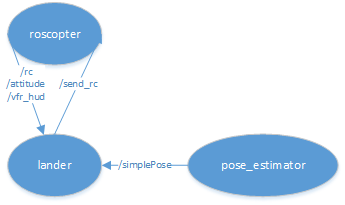
\includegraphics[width=.7\linewidth]{images/rosnodes.png}
  \caption{ROS nodes and topics for exchanging messages.}
  \label{fig:rosnodes}
\end{figure}

\textbf{OpenCV}, a computer vision library, is extremely popular and has considerable functionality relevant to this project. It also supports Video4Linux, a project to support common video capture devices in Linux. While other computer vision libraries exist, OpenCV is the most popular and hence is best supported online \cite{bestlibraryforcomputervision}.

Finally, we adapted \textbf{roscopter}, a compact ROS package that allows serial communication with devices supporting the MAVLink protocol (a standardised protocol used for communication to and from autonomous flight controllers or autopilots). This allows us to effect control over the autopilot from our co-computer.

\paragraph{Programming Language}
Our choice of programming language was guided by framework support and the need for performance when running on our boards. ROS has the most limited official support, having bindings for just C++ and Python. Given the known poor performance of embedded Python on ARM processors, our modules were implemented in C++.

\begin{figure*}
\centering
\begin{minipage}{.5\textwidth}
  \centering
  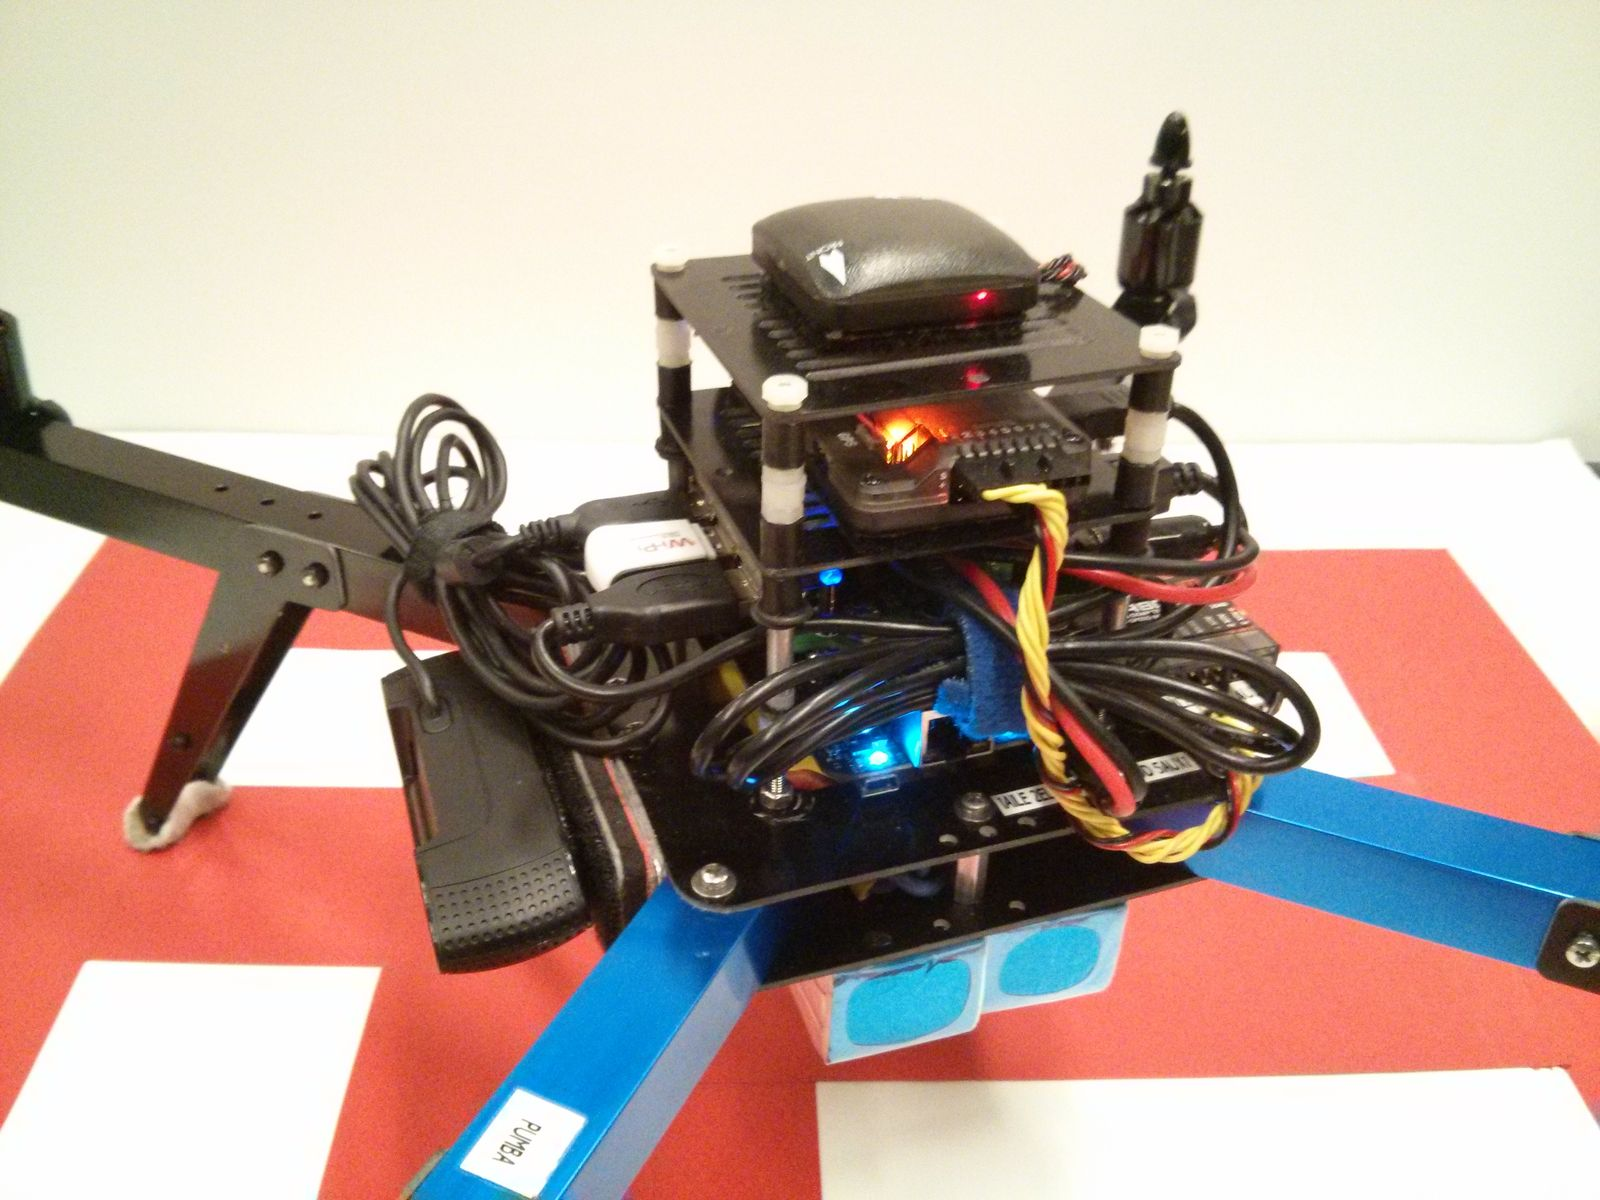
\includegraphics[width=.7\linewidth]{images/hardware.jpg}
  \captionof{figure}{Our hardware stack fully assembled. Total weight excluding batteries is 1.35 kg.} 
  \label{fig:hardware-photo}
\end{minipage}%
\begin{minipage}{.5\textwidth}
\centering
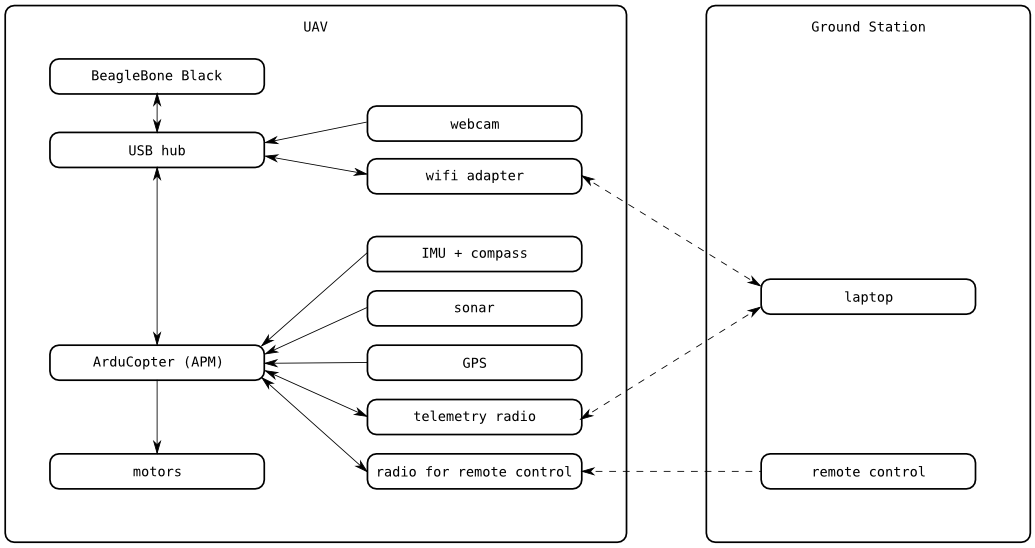
\includegraphics[width=0.9\textwidth]{images/architecture.png}
\captionof{figure}{Architecture of our automated landing system. We use inexpensive off-the-shelf hardware. All the computation is performed onboard the UAS.}
\label{fig:hardware-arch}
\end{minipage}
\end{figure*}

\subsection{Automated Landing}
The implemented automated landing system was based on the pose estimation algorithm described by Sharp et al. \cite{sharp_et_al_2001}. The following section describes our implementation of their approach and optimisations to it. 

\subsubsection{Landing Pad Design}
This particular algorithm requires the landing pad used for pose estimation to have a known pattern. In this case, our design is a monochromatic design consisting of five squares within a sixth, larger, square. The proportion of these squares to each other is known. For this pattern to be visible at higher altitudes, it must be large. Figure \ref{fig:corners} shows our landing pad and corner detection in action.


\begin{figure}[b]
    \centering
    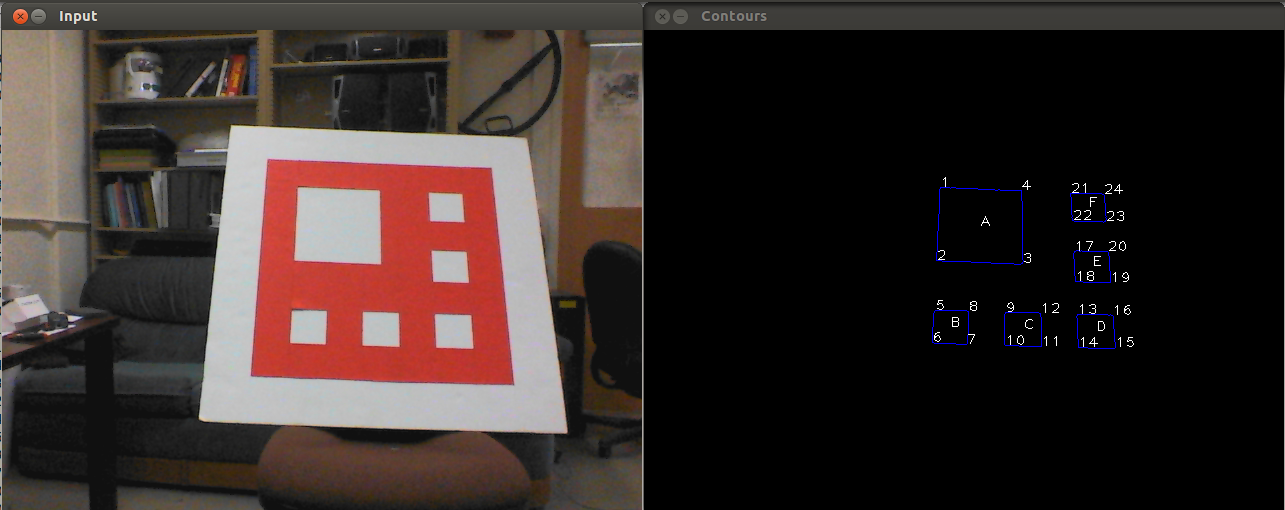
\includegraphics[width=0.9\linewidth]{images/corners.png}
    \caption{
        Left: Design of our landing platform.
        Right: Output of the corner detector (24 points, in order).
    }
    \label{fig:corners}
\end{figure}

\subsubsection{Vision Algorithm Overview}
The overall structure of our vision algorithm is shown in figure \ref{fig:flowchart-plain}.



\begin{figure*}[tb]
\centering
\begin{minipage}{.5\textwidth}
  \centering
  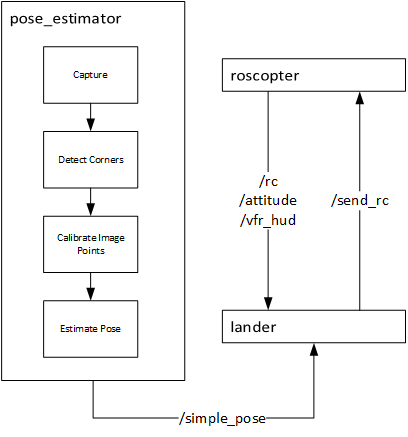
\includegraphics[width=.8\linewidth]{images/flowchart-plain.png}
  \captionof{figure}{Flowchart of overall algorithm.} 
  \label{fig:flowchart-plain}
\end{minipage}%
\begin{minipage}{.5\textwidth}
  \centering
  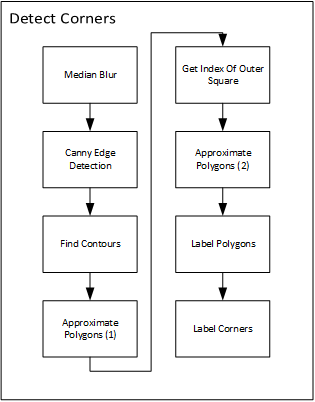
\includegraphics[width=.6\linewidth]{images/detectcorners-plain.png}
  \captionof{figure}{Flowchart of \textit{Detect Corners}.}
  \label{fig:detectcorners-plain}
\end{minipage}
\end{figure*}

\paragraph{Corner Detection}

As a first step, we detect the corners of the landing platform in an image, shown visually in figure \ref{fig:detectcorners-plain}:
\begin{enumerate}
\setlength{\itemsep}{0pt}
\setlength{\parskip}{0pt}
\setlength{\parsep}{0pt}
\item{
    \textbf{Median Blur, Canny Edge Detection} Denoise the image using a 3x3 median filter, and pass it through the Canny
    edge detector.}
\item{
    \textbf{Find Contours} Identify contours and establish a tree-structured hierarchy among them.}
\item{
    \textbf{Approximate Polygons} Discard contours which are not four-sided convex polygons and which have an
    area less than an experimentally determined threshold value.  We look for
    four-sided polygons and not specifically for squares, since they will not
    appear as squares under perspective projection.}
\item{
    \textbf{Get Index Of Outer Square} Using the contour hierarchy, determine a contour which contains 6 other
    contours. This contour represents the boundary of our landing platform.
    Store coordinates of the corners of these 6 inner contours.}
\item{
    \textbf{Label Polygons}  Label the largest of the 6 polygons as `A' and the farthest one from `A' as
    `D'. Label polygons as `B', `C', `E' and `F' based on their orientation and
    distance relative to the vector formed by joining centers of `A' and `D'.}
\item{
    \textbf{Label Corners} For each polygon, label corners in anti-clockwise order.}
\end{enumerate}

\paragraph{Pose Estimation}

We define the origin of the world coordinate frame to be the center of the
landing platform, such that all points on the landing platform have a Z
coordinate of zero. The corner detector gives us image coordinates for the 24
corners. Thus, we have a set of 24 point correspondences between world
coordinates and image coordinates. Given this input, we want to compute the
quadcopter's pose, i.e. the position and orientation of the camera in the world
coordinate frame. To do this, we followed the approach of Sharp et al.
 \cite{sharp_et_al_2001}, whose details are omitted here for brevity. We use SVD to
approximately solve a linear system of 48 equations with 6 degrees of freedom.

The output from the pose estimator is a translation vector
$t = \begin{bmatrix} t_x & t_y & t_z \end{bmatrix}^\top$
and a 3x3 rotation matrix $R$. We compute the camera position in world
coordinates as $C = -R^\top t$, and the yaw angle as
$\alpha = \arctan(R_{21} / R_{11})$. (The roll and pitch angles can be computed
similarly, but we do not require them in the control algorithm.)

The approach above assumes a calibrated pinhole camera. For the pose estimates
to be meaningful, our camera had to be calibrated first. We calibrated our
camera using the {\tt camera\_calibration} tool provided in the OpenCV
tutorials, plus some manual tuning. We used the resulting calibration matrix to
convert the raw pixel coordinates into coordinates for a calibrated pinhole
camera model, which we then fed into the equations above.

\subsubsection{Real-time Control}
In order to actually land a vehicle using these pose estimates, it was necessary to implement a high-level controller which worked in conjunction with the autopilot's own stabilisation modes. The state machine is more fully described in \cite{berzanaccurate}.

%%%%%%%%%%%%%%%%%%%%%%%%%%%%%%%%%%%%%%%%%%%%%%%%%%%%%%%%%%%%%%%%%%%%%%%%%%%%%%
\section{Approach\label{sec:approach}}

The naive implementation we began with operated at less than 3 frames per second on the BeagleBone Black. As mentioned previously, this is too slow for real-time control. This section describes the optimisations we made to our implementation to improve performance.

\subsection{Profiling}
We began by systematically profiling our code to identify hotspots where a disproportionate amount of time was being spent.  A full outline of our benchmarking technique is described in section \ref{sec:benchmarking}. At each stage of optimisation, we ran the pose estimation implementation through the same set of tests. Figure \ref{fig:flowchart-performance} shows hotspots inherent in our overall process and figure \ref{fig:detectcorners-performance} shows hotspots within the ``Detect Corners" subroutine. 


\begin{figure*}[t]
\centering
\begin{minipage}{.5\textwidth}
  \centering
  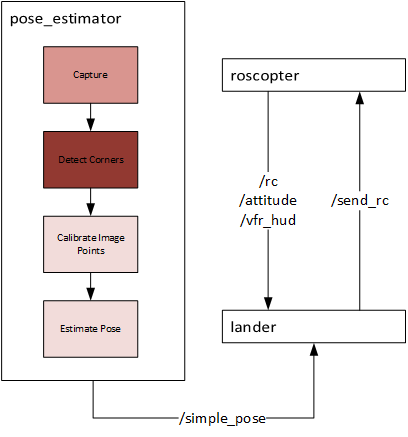
\includegraphics[width=.8\linewidth]{images/rosnodes-performance.png}
  \captionof{figure}{Flowchart of overall algorithm with hotspots highlighted.} 
  \label{fig:flowchart-performance}
\end{minipage}%
\begin{minipage}{.5\textwidth}
  \centering
  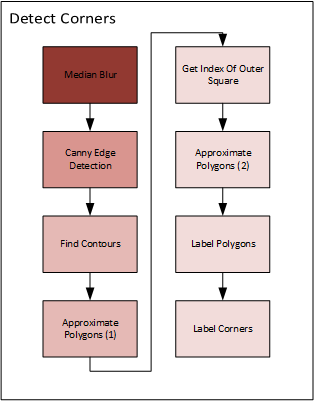
\includegraphics[width=.6\linewidth]{images/detectcorners-performance.png}
  \captionof{figure}{Flowchart of \textit{Detect Corners} with hotspots highlighted.}
  \label{fig:detectcorners-performance}
\end{minipage}
\end{figure*}


\subsection{Compiler Optimisations}
gcc and other compilers offer a myriad of optional performance optimisations. For example, they offer user specified flags that cause the generated executable file to be optimised for a certain instruction set. When compiling libraries such as OpenCV for an embedded computer, it is typical to cross-compile; compilation on embedded computers typically takes many times longer. Cross-compilation is when compilation happens on a more powerful compilation computer that has available to it a compiler for the target architecture. In our case, compilation was on a quad-core x86 computer for an ARM target architecture. At this stage, it is possible to pass certain parameters to the compiler that permit it to use ARM NEON instructions in the generated binary code.

NEON is an ``advanced SIMD instruction set" introduced in the ARMv7 architecture - the basis for all modern ARM processors. Single instruction, multiple data (SIMD) instructions are data parallel instructions that allow a single operation to be performed in parallel on two more operands. While the compiler has to be conservative in how it utilises these in the generated binary code so that correctness is guaranteed, these allow some performance gain.

Additionally, library providers may implement optional code paths that are enabled when explicitly compiling for an ARM target architecture. For instance, the OpenCV maintainers have several functions that have optional NEON instructions implemented. This also results in a performance boost.

\subsection{Library Optimisations}
OpenCV utilises other libraries to perform fundamental functions such as image format parsing and multi-threading. For core functions, such as parsing of image formats, a standard library is included and used. For advanced functions, support is optional and so these are disabled by default. 

We experimented with enabling multithreading functionality by compiling OpenCV with Intel's Thread Building Blocks library. This is a library that provides a multi-threading abstraction and for which support is available in select OpenCV functions \cite{opencvtbb}.

Secondly, we re-compiled OpenCV replacing the default JPEG parsing library, libjpeg, with a performance optimised variant called libjpeg-turbo. This claims to be 2.1 to 5.3x faster than the standard library \cite{libjpeg-turbo} and has ARM optimised code paths. Using this, it is possible to capture images at 30 frames per second on the BeagleBone Black \cite{bbb-30fps}.

Note also that we were unable to use the Intel Integrated Performance Primitives (IPP) library. IPP is the primary method of compiling a high performance version of OpenCV. However, it accomplishes this by utilising significant customisation for x86 processors that implement instruction sets only avaiable on desktop computers (e.g. Streaming SIMD Extensions (SSE), Advanced Vector Extensions (AVX)). 

\subsection{Single-threaded Optimisations}
We considered two approaches to optimise our single-threaded implementation. Since the BeagleBone Black uses a single core processor, multi-threading is unlikely to have resulted in significant performance gains and so it was important to optimise the single-threaded version as much as possible to extract better performance from this board. 

An obvious optimisation to our initial approach was to identify function calls and substeps that were unnecessary. Through benchmarking, we attempted to remove or reduce the impact of calls which were taking a significant amount of processing time. At each stage, we ensured that robustness to image quality was retained by testing against approximately 6,000 images captured in the lab and in the air. We describe the nature of these changes in the next section.

A second optimisation was to try and increase processor level parallelism (as opposed to the operating system parallelism that threading would provide). As mentioned previously, modern ARM processors implement the NEON SIMD instruction set. Compilers such as gcc make instruction set specific SIMD instructions available to the programmer through additional instructions called intrinsics. Intrinsics essentially wrap calls to the underlying SIMD instruction.

Using intrinsics, it is possible to exploit data parallelism in our own code, essentially rewriting higher level, non-parallel, function calls with low level function calls that operate on multiple data simultaneously. This approach is laborious and is therefore used sparingly. It can, however, yield significant performance improvements \cite{mitra2013use}. Our initial attempt at rewriting computer vision functions using intrinsics were actually slower and time constraints prevented us from investigating this. Therefore, results from our own SIMD implementation are omitted.

\subsection{Multi-threaded Optimisations}
Multi-threading is a promising approach. Certain library functions may inherently exploit multi-threading and there is a slight benefit to a single-threaded process to having multiple cores (the operating system will balance processes across cores). However, our single-threaded implementation still gains little performance from having multiple cores available - many of which were not occupied with useful work. 

Our multi-threaded implementation separates out the \textbf{Capture} step from the latter \textbf{Detect Corners}, \textbf{Calibrate Image Points} and \textbf{Estimate Pose} steps as shown in figure \ref{fig:flowchart-multi}. This is accomplished by creating a pool of worker threads (the exact quantity of threads is configurable - generally 1 for every available core). Each time an image is captured, it is dispatched to the next free thread in a round-robin fashion. Work is distributed evenly across threads and, since each thread finishes computation of images in a similar time, pose estimates are published to the \textit{\textbackslash simplePose} topic in order of image acquisition.  This approach is essentially \textbf{pipelining}, each thread can be considered a pipeline, allowing concurrent processing of an image while the master thread captures the next image.  Figure \ref{fig:pipelining} shows how frames are processed for a single threaded process above that for a pipelined multi-threaded process.

\begin{figure}[ht!]
    \centering
    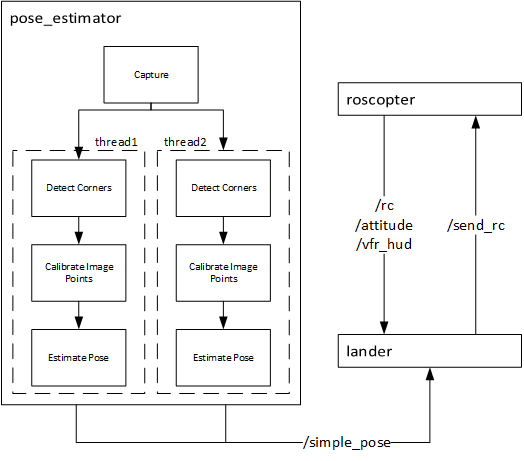
\includegraphics[width=\linewidth]{images/flowchart-plain-multi-threaded.png}
    \caption{Refactored ROS nodes to allow multi-threading.}
    \label{fig:flowchart-multi}
\end{figure}

We use the POSIX thread (pthread) libraries to assist with thread creation and management.

\begin{figure*}[tb]
    \centering
    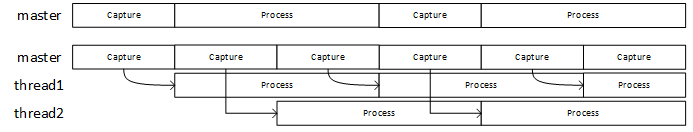
\includegraphics[width=0.9\textwidth]{images/pipelining.png}
    \caption{}
    \label{fig:pipelining}
\end{figure*}


%%%%%%%%%%%%%%%%%%%%%%%%%%%%%%%%%%%%%%%%%%%%%%%%%%%%%%%%%%%%%%%%%%%%%%%%%%%%%%
\section{Results\label{sec:results}}

\subsection{Benchmarking Methodology \label{sec:benchmarking}}
\paragraph{Environment} The large fixed size landing pad was used a fixed distance of approximately 1.5 meters from the web camera. All tests were performed indoors in a room without windows and with a constant lighting level produced by a fluorescent tube light. No other user space processes were running on each computer aside from \textit{roscore} and the pose estimator process itself. 

\paragraph{Timing Data} Each implementation was benchmarked using calls to C++'s \textit{gettimeofday} function. For each implementation we profiled the amount of time taken for various calls within our pose estimation routine over 20 frames. For each test, we discarded the first 20 frame chunk since this is when the camera automatically adjusts exposure and focus settings. This data was collected for 10 arbitrary 20 frame chunks and averaged to provide overall figures.

\subsection{Maximum Performance}
The Logitech C920 web camera we are using captures frames at a 640 x 480 pixel resolution at a maximum of 30 frames per second. It would be impossible to operate any quicker than the camera is capable of delivering frames and therefore the upper bound for performance is 30 Hz.

\begin{table}[htbp]
  \centering
    \begin{tabular}{rrr}
    \toprule
    \textbf{Board} & \textbf{BeagleBone} & \textbf{Odroid} \\
    \midrule
    No computation & 29.57 & 29.65 \\
    Basic decoding using OpenCV & 18.69 & 24.60 \\
    \bottomrule
    \end{tabular}%
    \caption{Baseline FPS for the BeagleBone and Odroid boards.}
 \label{tab:baseline}
\end{table}%

Using the framegrabber.c application provided in \cite{bbb-30fps}, it was possible to evaluate what the maximum single threaded performance could be, assuming basic decoding of image frame using OpenCV and no other computation. Table \ref{tab:baseline} shows the results of this benchmark. We see that the BeagleBone performs at 75\% of the speed of the Odroid - which is intuitively correct, given the slower clock speed of the BeagleBone's processor and the fact that it has just a single core - some amount of its load will be used by operating system tasks that can be scheduled on other cores on the Odroid. 

\subsection{Performance of Naive Implementation}
To begin with, we benchmarked our naive implementation with no optimisations on both boards and a desktop computer with a quad-core Intel Core i5 processor. This showed an obvious discrepancy in performance, with average FPS for each shown in table \ref{tab:naive-all-fps}.

\begin{table}[htbp]
  \centering
    \begin{tabular}{rrr}
    \toprule
    \multicolumn{1}{c}{\multirow{2}[1]{*}{Board}} & \multicolumn{2}{c}{Pad visible} \\
    \multicolumn{1}{c}{} & \multicolumn{1}{c}{no} & \multicolumn{1}{c}{yes} \\
    \midrule 
    \multicolumn{1}{l}{BeagleBone} & 2.94  & 3.01 \\
    \multicolumn{1}{l}{Desktop} & 30.04 & 29.97 \\
    \multicolumn{1}{l}{Odroid} & 8.80  & 8.93 \\
    \bottomrule
    \end{tabular}%
   \caption{Naive implementation: average FPS for the BeagleBone, Odroid and a desktop computer.}%
  \label{tab:naive-all-fps}%
\end{table}%


The desktop computer has no issue running at the maximum 30 FPS but both the BeagleBone and Odroid fail to give the necessary 10 Hz required for real-time control (as described in section \ref{sec:optimisation-techniques}). 

There is a slight but obvious discrepancy between performance when the pad is in view and when the pad is not which only appears to manifest itself on the two ARM boards (the BeagleBone and Odroid). By profiling the steps of detect corners, the first four of which are shown for the Odroid in table \ref{tab:naive-frame-vs-no-frame}, we can begin to see why. Canny edge detection and finding contours takes very slightly longer on both boards when there is no pad in view. Intuitively this is because when the pad is in view, it occludes a significant part of the image. The pad is constructed of very simple quadrilaterals that are atypical of the many small heterogeneous shapes that a normal frame is composed of. For the remaining tests the figures represent performance when the pad is in view.

% Table generated by Excel2LaTeX from sheet 'Naive'
\begin{table*}[htbp]
  \centering
    \begin{tabular}{ccccc}
    \toprule
    \textbf{Pad} & \textbf{Median Blur} & \textbf{Canny} & \textbf{Find Contours} & \textbf{Approximate Polygons (1)} \\
    \midrule
    No    & 0.054 & 0.039 & 0.003 & 0.001 \\
    Yes   & 0.054 & 0.038 & 0.002 & 0.001 \\
    \bottomrule
    \end{tabular}%
  \caption{Naive implementation: breakdown of first four steps of \textit{Detect Corners} with and without a frame in view for Odroid (similar results for BeagleBone).}%
  \label{tab:naive-frame-vs-no-frame}%
\end{table*}%
 
Figure \ref{fig:naive-breakdown-overall} show a breakdown of the naive implementation of the overall algorithm on all three of our boards. It is clear that the majority of time is spent in the \textit{Capture} and \textit{Detect Corners} stages. Video capture is handled by an OpenCV function so we are unable to easily profile that. However, figure \ref{fig:naive-breakdown-detect-corners} shows a breakdown of time spent in the \textit{Detect Corners} subroutine. Again, here, it is clear that two calls to \textit{Median Blur} and \textit{Canny} contribute the majority of processing time.


\begin{figure*}[htbp]
\centering
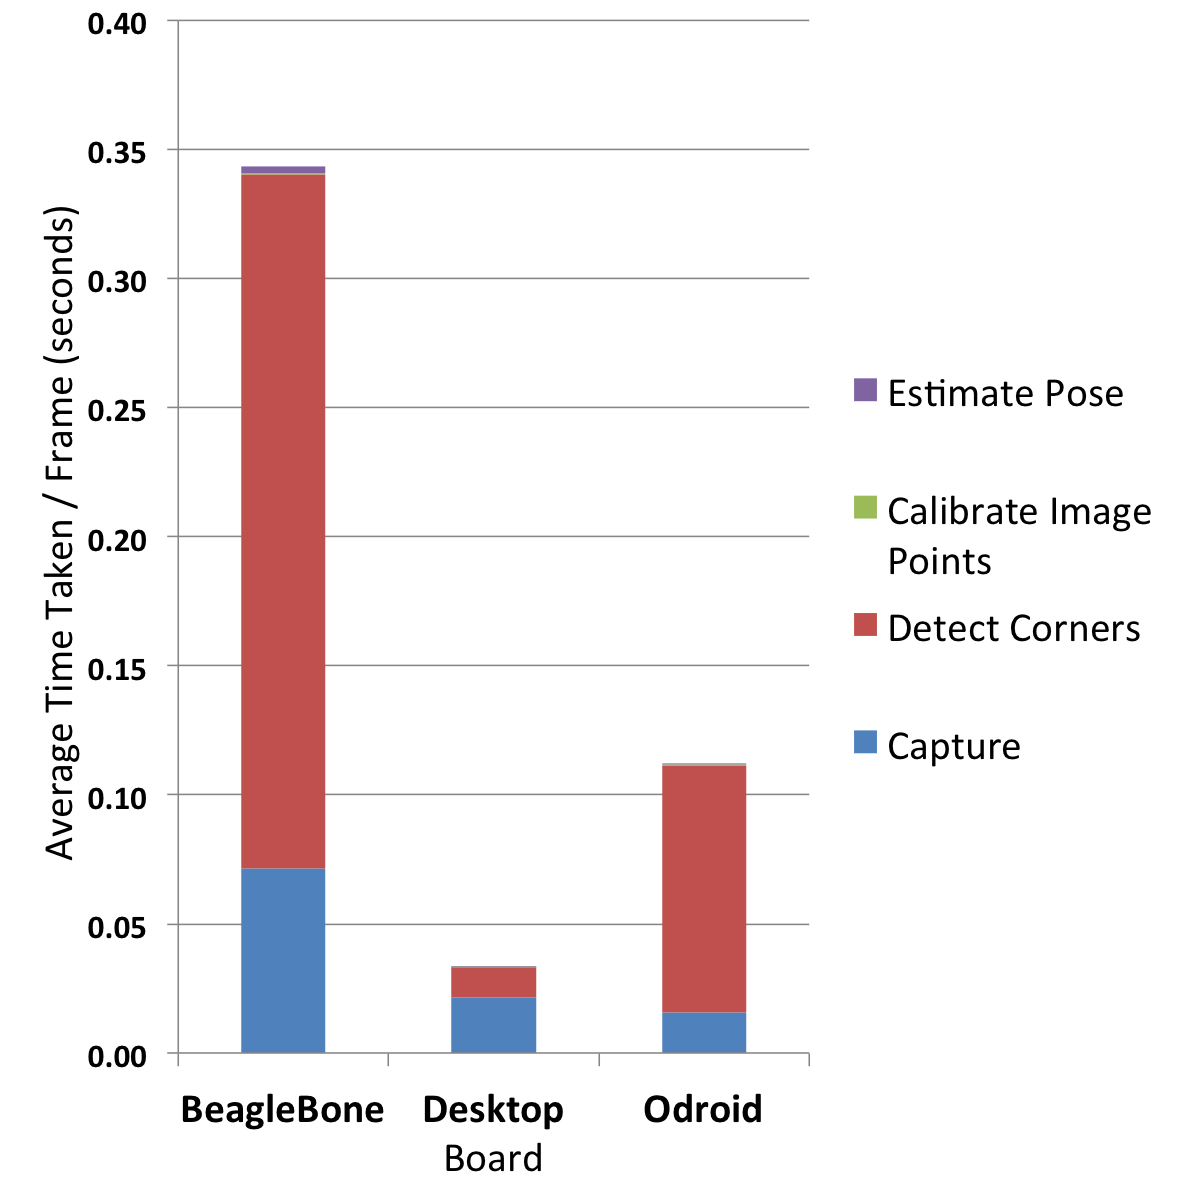
\includegraphics[height=0.43\textheight]{images/performance/naive-breakdown-overall.png}
\captionof{figure}{Naive implementation: \\ breakdown of overall algorithm} 
\label{fig:naive-breakdown-overall}
\end{figure*}

\begin{figure*}[htbp]
\centering
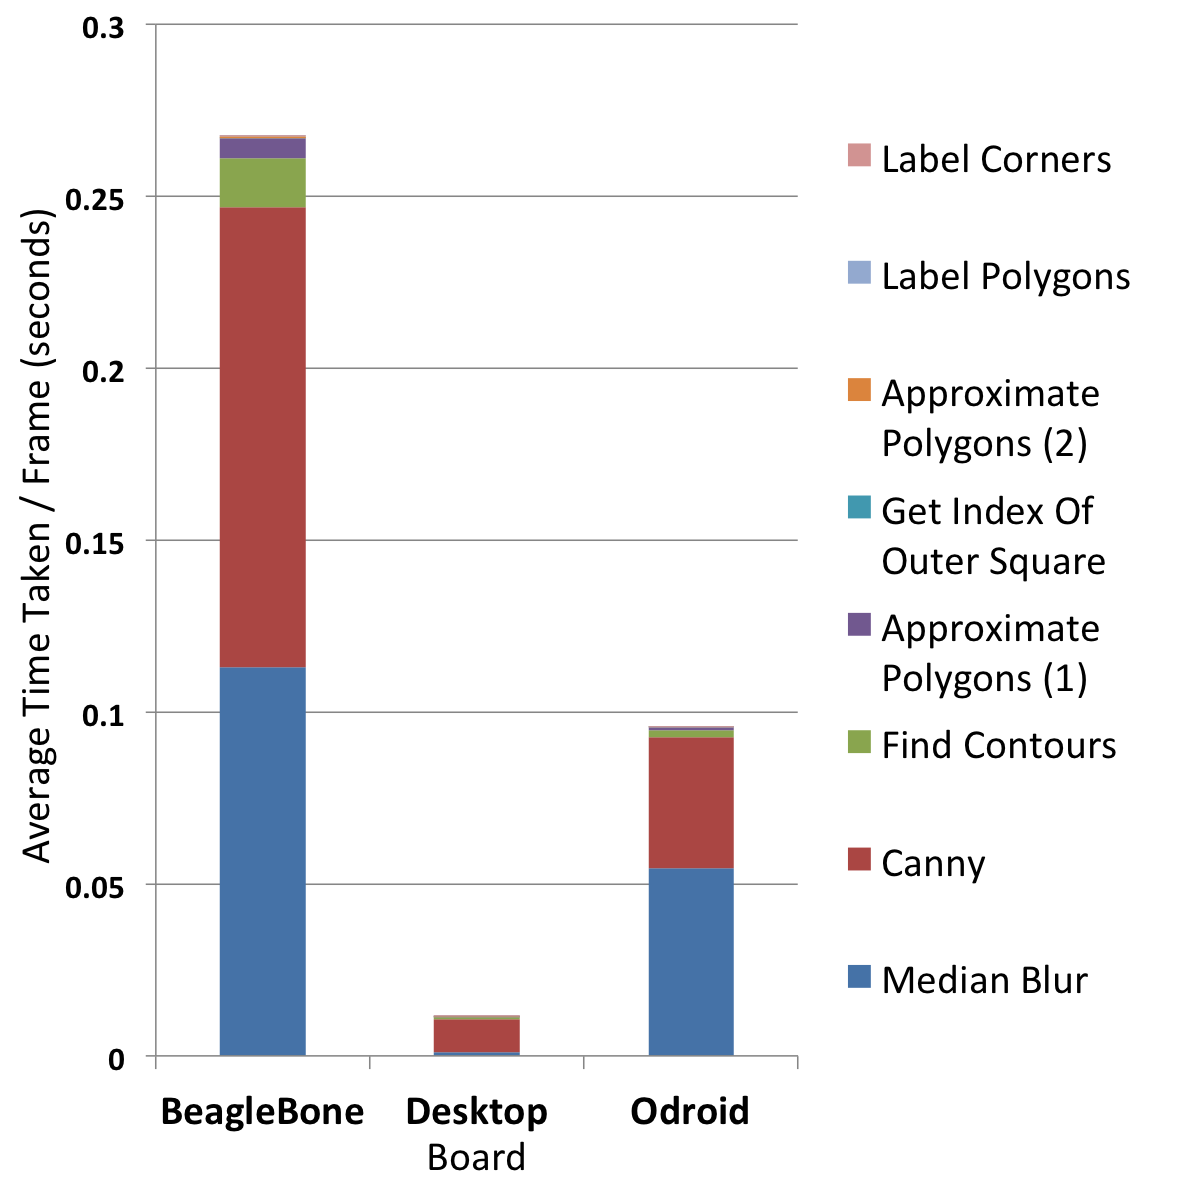
\includegraphics[height=0.43\textheight]{images/performance/naive-breakdown-detect-corners.png}
\captionof{figure}{Naive implementation: \\ breakdown of \textit{Detect Corners}}
\label{fig:naive-breakdown-detect-corners}
\end{figure*}


\subsection{Performance of Naive Implementation with Optimised Libraries}


The next stage of optimisation was to adapt the libraries used onboard. OpenCV was the primary focus and we did three things, as described in \ref{sec:compiler-opt}:
\begin{enumerate}
\setlength{\itemsep}{0pt}
\setlength{\parskip}{0pt}
\setlength{\parsep}{0pt}
\item{Cross compile with NEON code generation enabled}
\item{Cross compile with NEON code generation and Thread Building Blocks (TBB) support enabled}
\item{Cross compile with NEON code generation, TBB support and libjpeg-turbo support enabled}
\end{enumerate}

Table \ref{tab:library-optimisations} shows the improvement in average FPS for each adapation. We get overall a 10\% gain in performance over the standard library.  Note that the addition of Thread Building Blocks does very little for performance because the OpenCV functions used were not optimised to use it.

% Table generated by Excel2LaTeX from sheet 'Compiler Flags'
\begin{table*}[htbp]
  \centering
  
    \begin{tabular}{rrrrr}
    \toprule
    \textbf{Board} & \textbf{Standard} & \textbf{NEON} & \textbf{NEON+TBB} & \textbf{NEON+TBB+libjpeg-turbo} \\
    \midrule
    \multicolumn{1}{l}{BeagleBone} & 2.91  & 2.84  & 2.98  & 3.20 \\
    \multicolumn{1}{l}{Odroid} & 8.93  & 9.60  & 9.60  & 9.90 \\
    \bottomrule
    \end{tabular}%
  \caption{Naive implementation with optimised libraries: average FPS for the BeagleBone and Odroid with various library optimisations.}
  \label{tab:library-optimisations}%
\end{table*}%


Figure \ref{fig:libraries-breakdown-overall} shows how the time taken for steps in the overall algorithm changes with each adaptation. Compiling for the NEON architecture causes consistent gains across each procedure while using libjpeg-turbo specifically optimises the \textit{Capture} step. This can be explained by the fact that the \textit{Capture} is frame data encoded in Motion-JPEG from the web camera into the \textbf{Mat} object OpenCV uses internally.

\begin{figure*}[htbp]
\centering
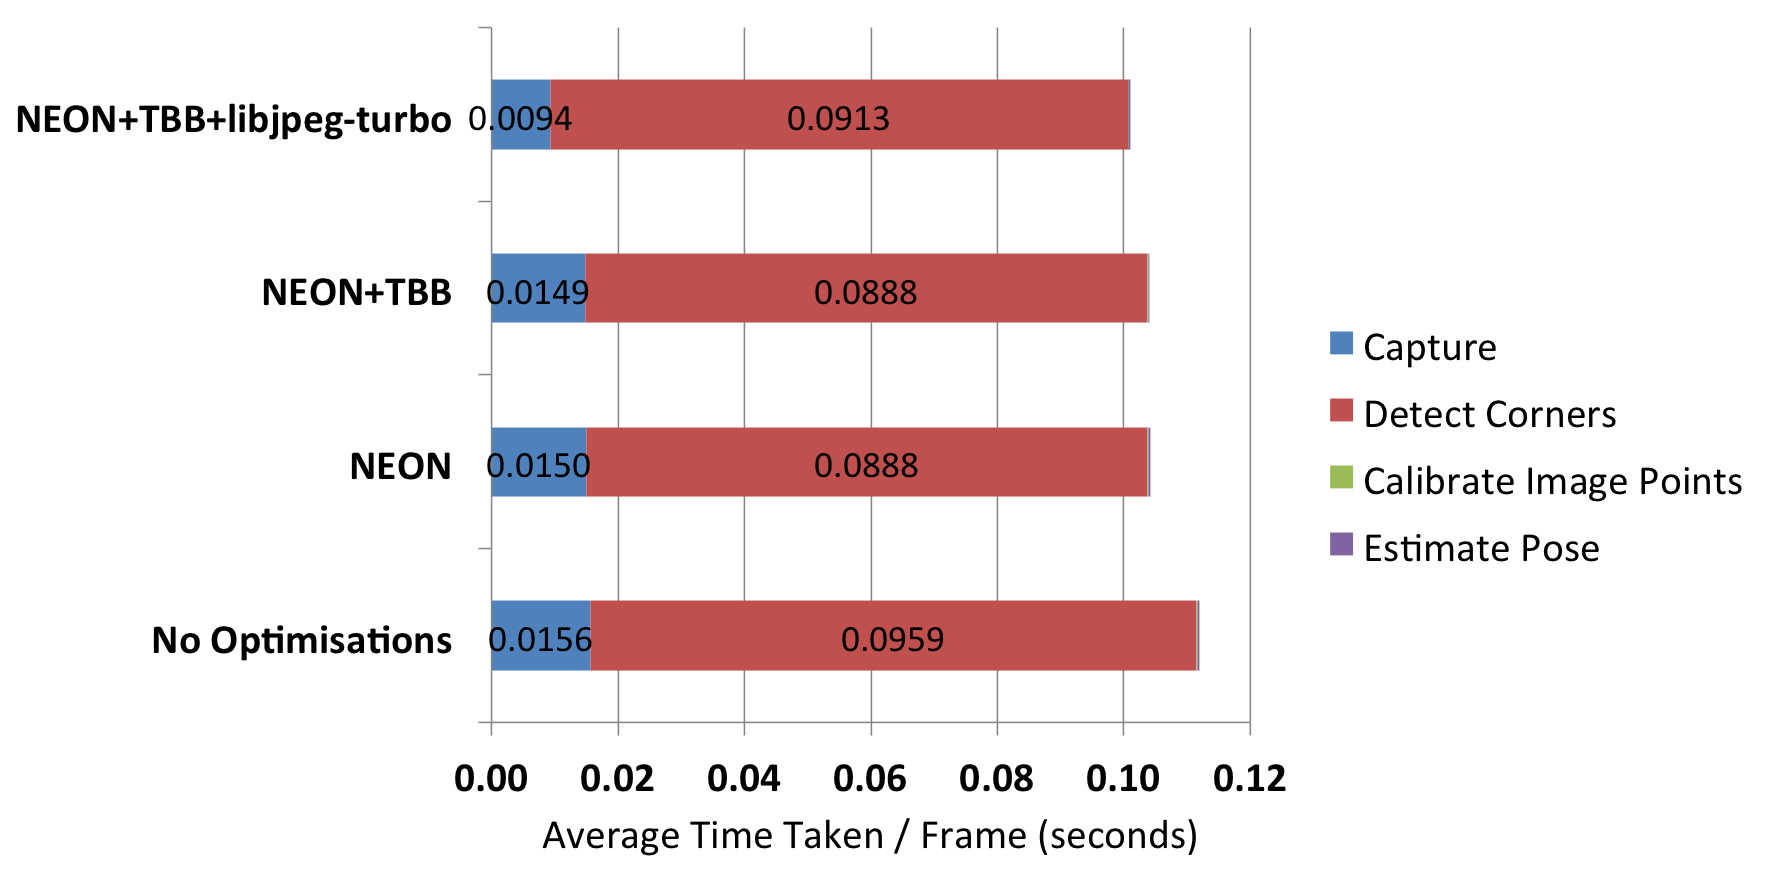
\includegraphics[width=\textwidth]{images/performance/libraries-breakdown-overall.png}
\caption{Naive implementation with optimised libraries: breakdown of overall algorithm for Odroid (similar results for BeagleBone).}
\label{fig:libraries-breakdown-overall}
\end{figure*}

\subsection{Performance of Single-threaded Optimised Implementation}

Our first optimisation to the code itself was to remove redundant calls and to minimise computation whereever possible. It turns out that the \textit{Median Blur} step within the \textit{Detect Corners} subroutine was unnecessary. Furthermore, some of our loops used to detect polygons would operate on all contours detected and not just those of interest. This led to extra unnecessary computation.  


Figure \ref{fig:single-opt-breakdown-detect-corners} shows how the time taken by each stage of \textit{Detect Corners} before and after this change.


Table \ref{tab:single-threaded-optimisation-bb-odroid-fps} shows the performance improvement of approximately 60\% when run on the BeagleBone and 120\% when run on the Odroid. 

% Table generated by Excel2LaTeX from sheet 'Single Threaded Opt'
\begin{table*}[htbp]
  \centering
    \begin{tabular}{rrr}
    \toprule
    \textbf{Board} & \textbf{Optimised Libraries} & \textbf{Optimised Single Threaded} \\
    \midrule
    \multicolumn{1}{l}{BeagleBone} & 3.20  & 5.08 \\
    \multicolumn{1}{l}{Odroid} & 9.90  & 21.58 \\
    \bottomrule
    \end{tabular}%
  \caption{Single-thread optimised implementation: average FPS for the BeagleBone and 
  Odroid}
  \label{tab:single-threaded-optimisation-bb-odroid-fps}%
\end{table*}%


\begin{figure*}[htbp]
\centering
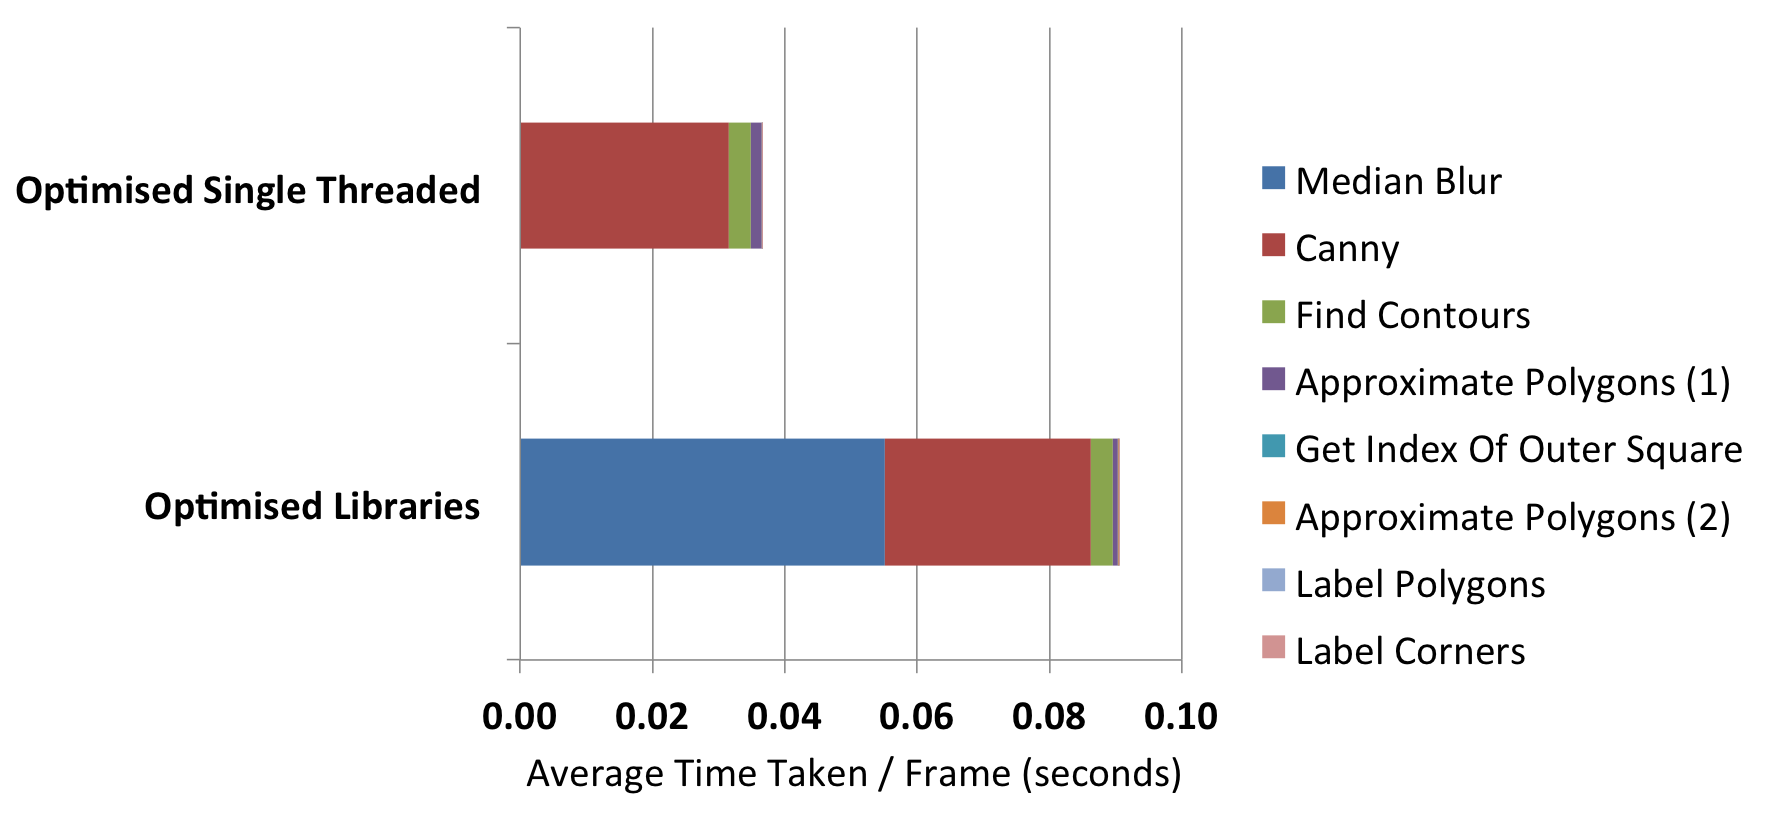
\includegraphics[width=\textwidth]{images/performance/single-opt-breakdown-detect-corners.png}
\caption{Single-thread optimised implementation: breakdown of \textit{Detect Corners} for Odroid (similar results for BeagleBone).}
\label{fig:single-opt-breakdown-detect-corners}
\end{figure*}


\subsection{Performance of Multi-threaded Optimised Implementation}

The next optimisation implemented was pipelining by using multiple threads. Profiling data was collected for 1, 2, 4 and 8 threads and compared to the baseline single-threaded optimised version. 

Figures \ref{fig:multi-opt-beaglebone-fps} and \ref{fig:multi-opt-odroid-fps} shows this for the BeagleBone and Odroid respectively. Performance suffers significantly on the BeagleBone, a single core board, as context switching causes extra overhead. This context switching is visible when using a single thread on the Odroid (because of context switching between the master thread and the single worker thread) but the performance benefit becomes clear as additional threads are introduced.

2 threads appears sufficient to get us to almost 30 frames per second - with the occasional frame not getting processed due to fully loaded worker threads. With 3 or more worker threads, no frame gets lost.

\begin{figure*}[htbp]
\centering
\begin{minipage}{.5\textwidth}
  \centering
  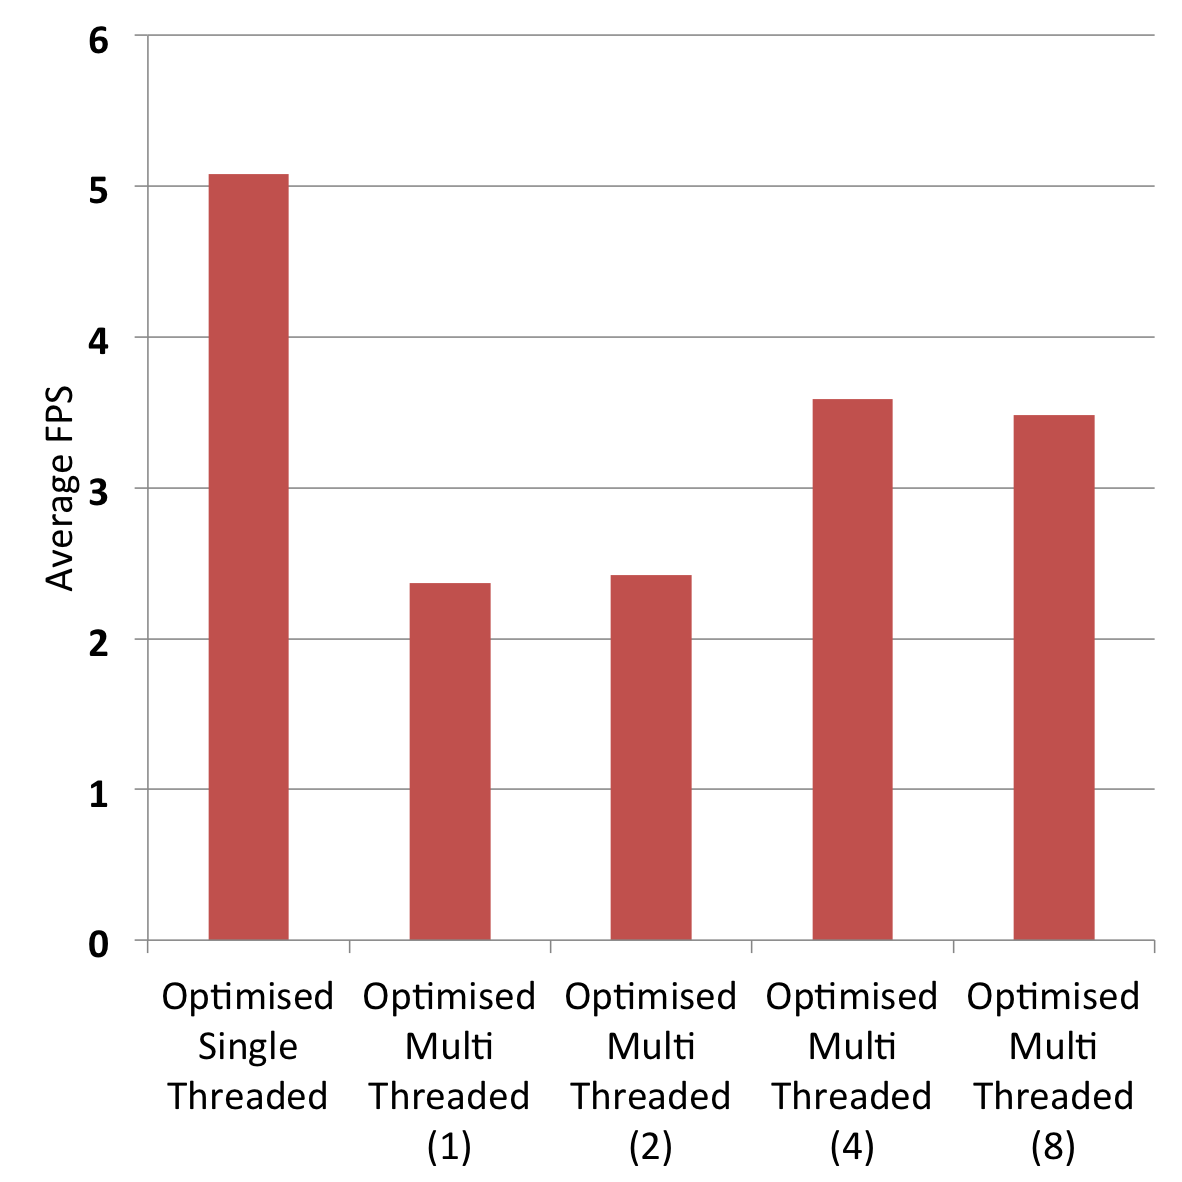
\includegraphics[width=\textwidth]{images/performance/multi-beaglebone-fps.png}
  \captionof{figure}{Multi-thread optimised implementation: \\ average FPS for BeagleBone for different numbers of threads} 
  \label{fig:multi-opt-beaglebone-fps}
\end{minipage}%
\begin{minipage}{.5\textwidth}
  \centering
  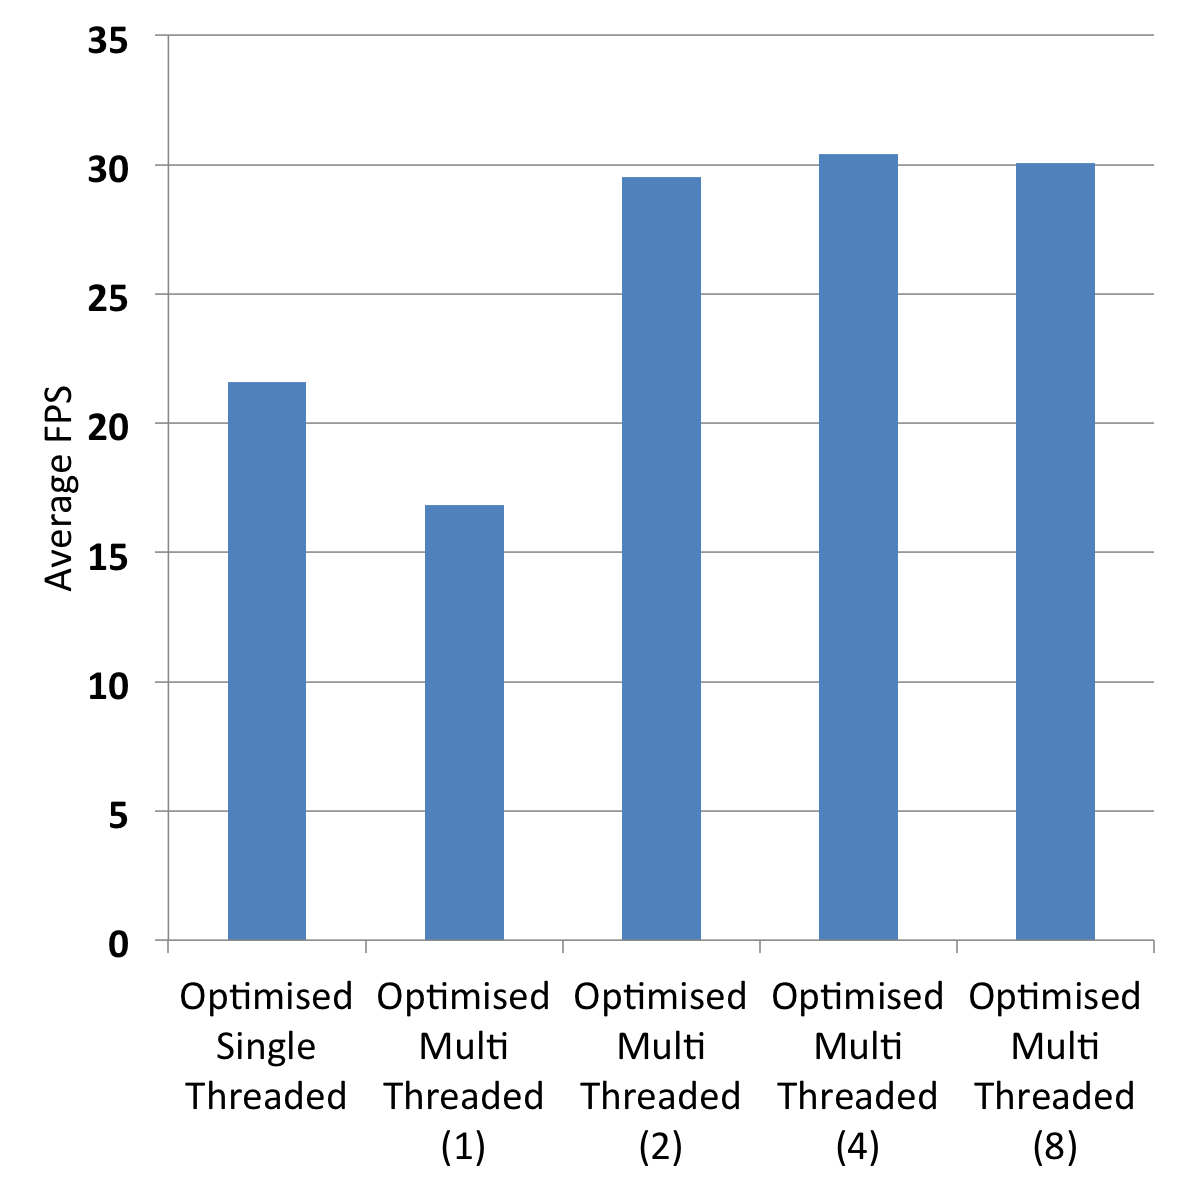
\includegraphics[width=\textwidth]{images/performance/multi-odroid-fps.png}
  \captionof{figure}{Multi-thread optimised implementation: \\ average FPS for Odroid for different numbers of threads}
  \label{fig:multi-opt-odroid-fps}
\end{minipage}
\end{figure*}

Table \ref{tab:multi-opt-odroid-load} shows the 1 minute average system load (also known as the number of waiting processes) reported by Linux as additional threads are added when running on the Odroid. This does not increase significantly beyond 2 threads, validating the earlier point that 2 threads is sufficient to carry out nearly all of the computation.

% Table generated by Excel2LaTeX from sheet 'Multi Threaded Opt'
\begin{table}[htbp]
  \centering
  
    \begin{tabular}{cc}
    \toprule
    \textbf{Threads} & \textbf{System Load} \\
    \midrule
    1     & 0.59 \\
    2     & 1.10 \\
    4     & 1.17 \\
    8     & 1.20 \\
    \bottomrule
    \end{tabular}%
  \caption{Multi-thread optimised implementation: 1 minute average system load for Odroid for different numbers of threads}
  \label{tab:multi-opt-odroid-load}%
\end{table}%

\subsection{Performance of Single-threaded Optimised Implementation (2)}

When it became clear that our initial single-threaded optimised implementation was not working quickly enough on the BeagleBone and when multi-threading failed to work, we re-visited the single-threaded approach and looked for alternative approaches to computation.

By replacing \textit{Canny Edge Detection} by adaptive thresholding, we were able to improve the performance of our single-threaded implementation further to almost 6 FPS on the BeagleBone and to the maximum 30 FPS on the Odroid. The pose estimation results remain correct.

Table \ref{tab:single-threaded-optimisation-2-fps} shows the improvement in FPS over our original single-threaded optimised implementation.

% Table generated by Excel2LaTeX from sheet 'Single Threaded Opt (2)'
\begin{table*}[htbp]
  \centering
    \begin{tabular}{rrr}
    \toprule
    \textbf{Board} & \textbf{Optimised Single Threaded} & \textbf{Optimised Single Threaded (2)} \\
    \midrule
    \multicolumn{1}{l}{BeagleBone} & 5.08  & 5.97 \\
    \multicolumn{1}{l}{Odroid} & 21.58 & 30.19 \\
    \bottomrule
    \end{tabular}%
  \caption{Single-thread optimised implementation (2): average FPS for the BeagleBone and Odroid}%
  \label{tab:single-threaded-optimisation-2-fps}%
\end{table*}%

Figure \ref{fig:single-opt-2-breakdown-detect-corners} shows that the majority of the speed increase came from the reduction in time taken by the \textit{Canny Edge Detection} step. There was also a corresponding time saving during the \textit{Find Contours} step - presumably because thresholding is actually a more selective preprocessing method than Canny edge detection.

\begin{figure*}[htbp]
\centering
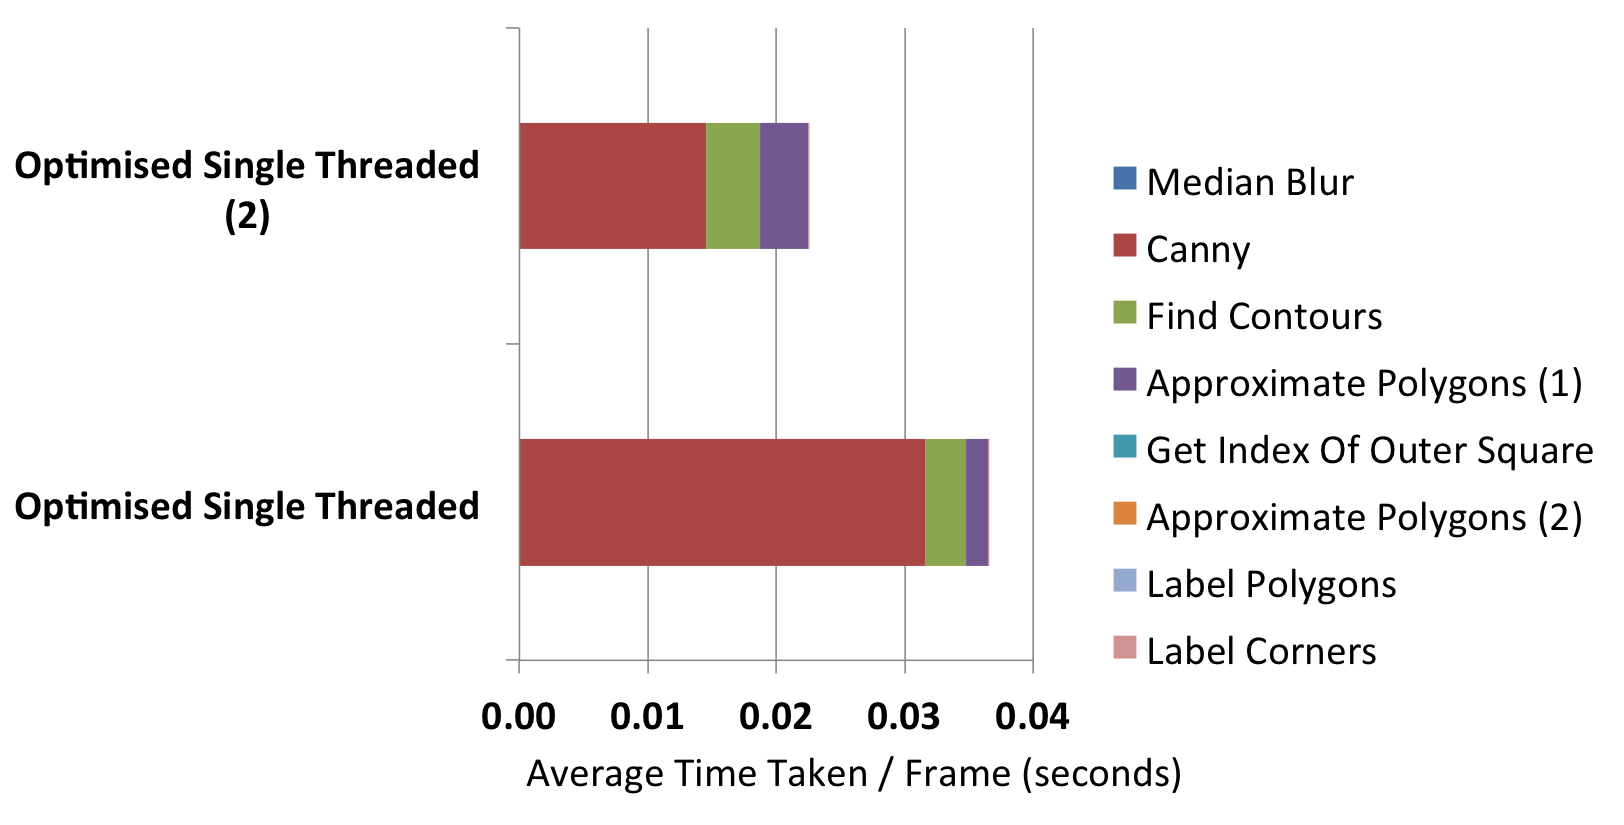
\includegraphics[width=\textwidth]{images/performance/single-opt-2-breakdown-detect-corners.png}
\caption{Single-thread optimised implementation 2: breakdown of \textit{Detect Corners} for Odroid (similar results for BeagleBone).}
\label{fig:single-opt-2-breakdown-detect-corners}
\end{figure*}

\subsection{Performance Summary}
Figures \ref{fig:beaglebone-fps} and \ref{fig:odroid-fps} show the increase in average FPS for each of the implementations as various optimisations were added. Our best performance was just under 6 FPS for the BeagleBone and at the full 30 FPS for the Odroid. Figure \ref{fig:best-to-worst-detect-corners} shows the difference in processing time for each frame in \textit{Detect Corners} frmo the naive implementation to the optimised single threaded version. Notice that our optimisations made a proportionally greater difference on the Odroid than the BeagleBone.

\begin{figure*}[h]
\centering
\begin{minipage}{.5\textwidth}
  \centering
  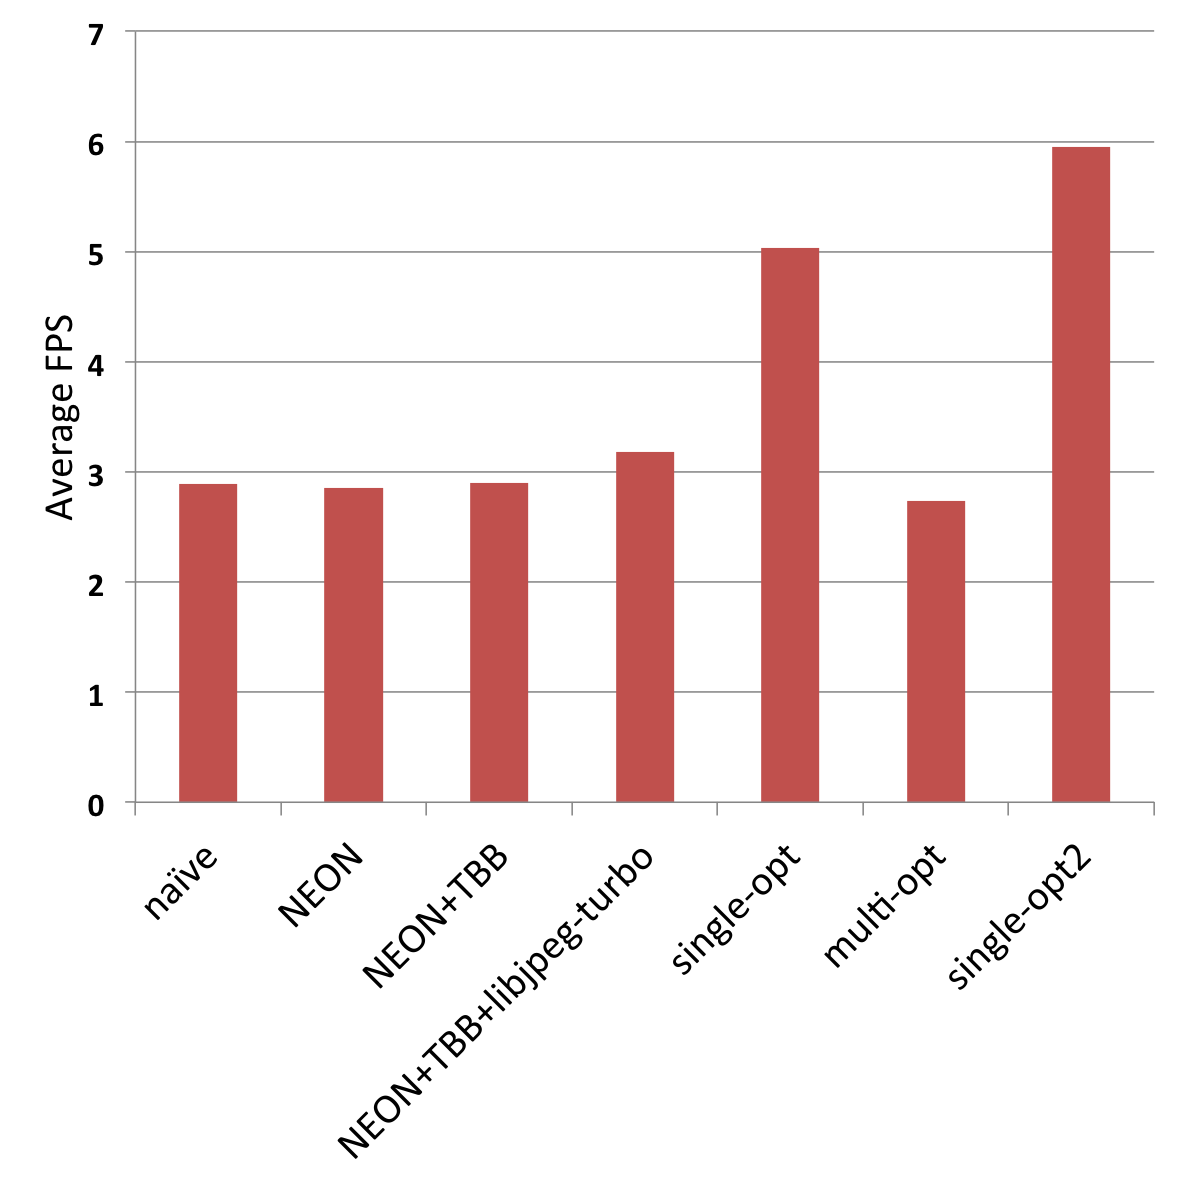
\includegraphics[width=\textwidth]{images/performance/beaglebone-fps.png}
  \captionof{figure}{All implementations: \\ average FPS for BeagleBone} 
  \label{fig:beaglebone-fps}
\end{minipage}%
\begin{minipage}{.5\textwidth}
  \centering
  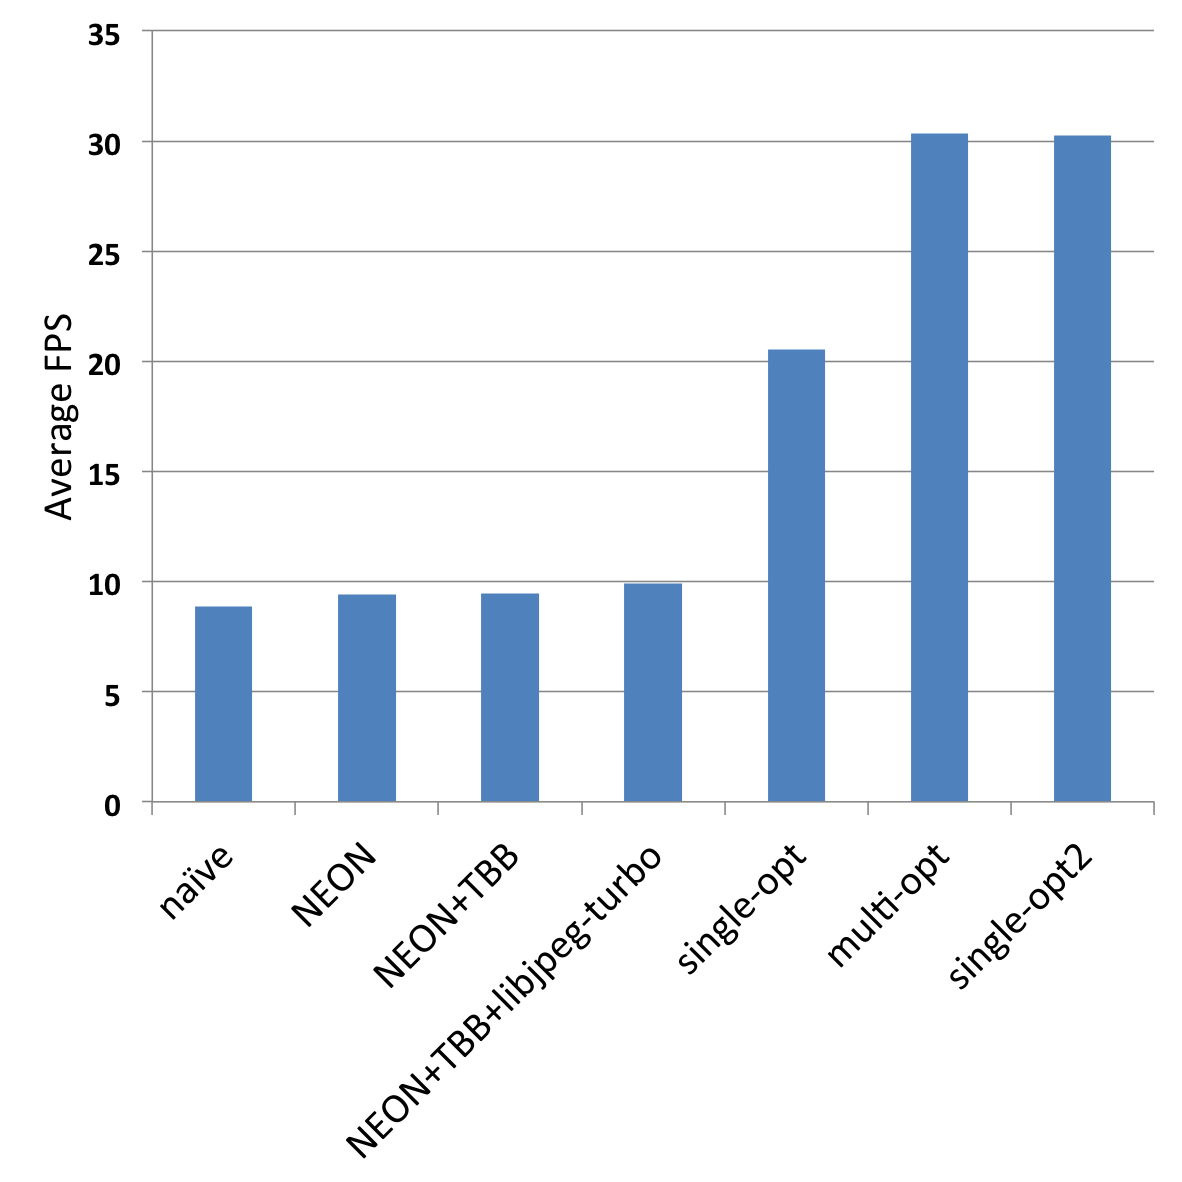
\includegraphics[width=\textwidth]{images/performance/odroid-fps.png}
  \captionof{figure}{All implementations: \\ average FPS for Odroid}
  \label{fig:odroid-fps}
\end{minipage}
\end{figure*}

\begin{figure*}[h]
\centering
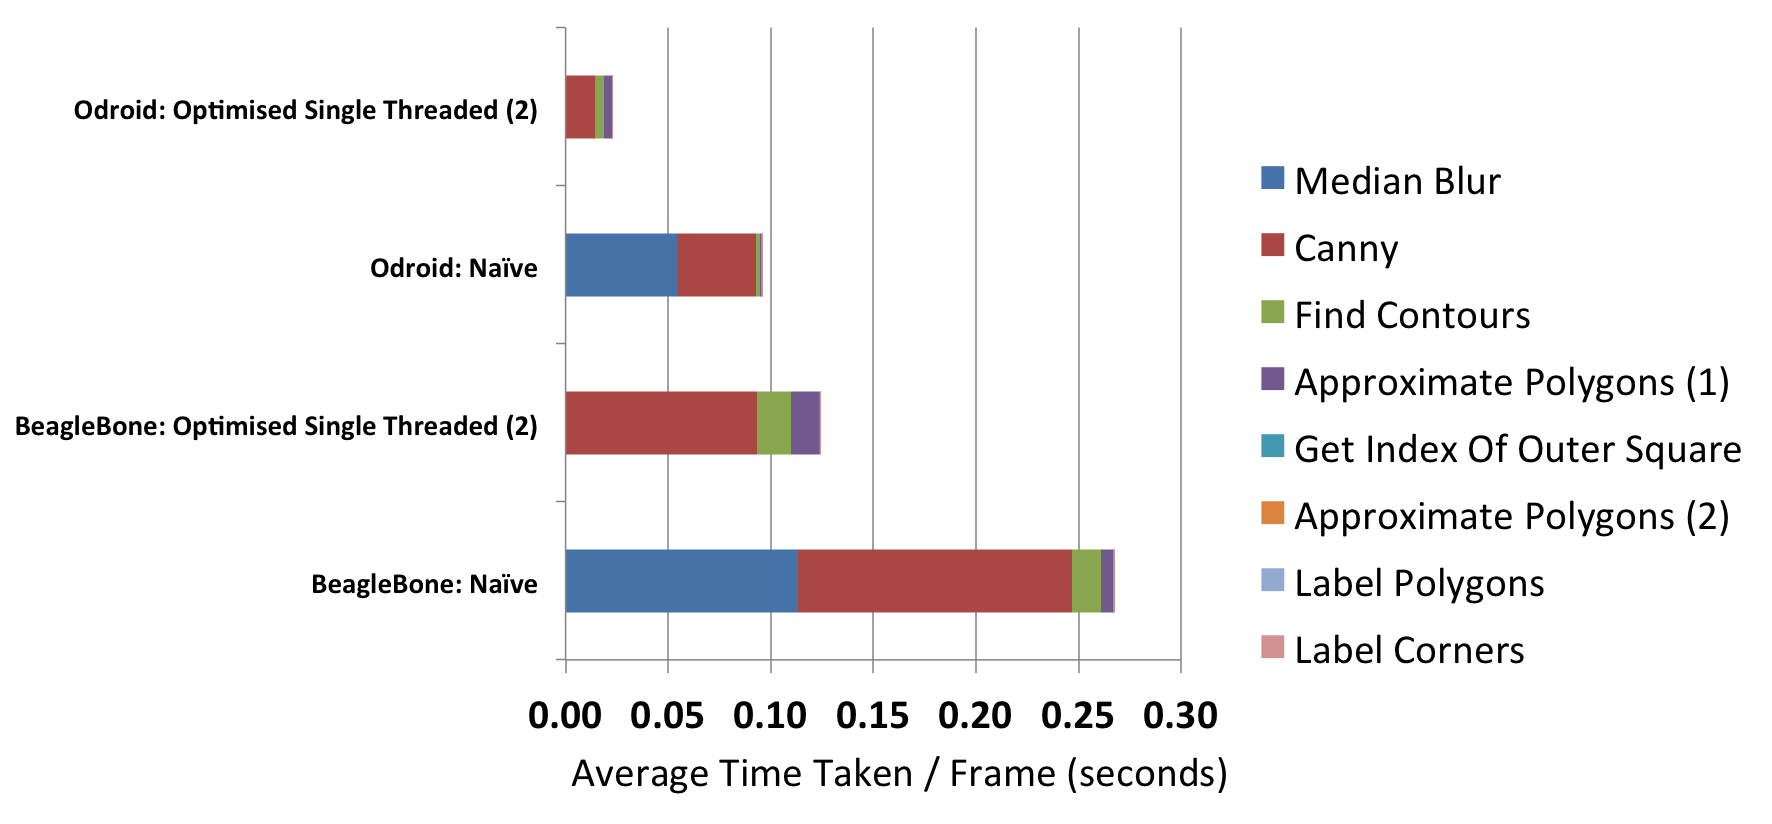
\includegraphics[width=\textwidth]{images/performance/worst-to-best-detect-corners.png}
\caption{Naive to optimised implementation: breakdown of \textit{Detect Corners} for BeagleBone and Odroid.}
\label{fig:best-to-worst-detect-corners}
\end{figure*}

%%%%%%%%%%%%%%%%%%%%%%%%%%%%%%%%%%%%%%%%%%%%%%%%%%%%%%%%%%%%%%%%%%%%%%%%%%%%%%
\section{Conclusion}
In 2011, Sharp et al \cite{sharp_et_al_2001} reported results of 30 FPS while running this pose estimation algorithm.  They used highly optimised custom C code running on a much slower board and took significantly more time to implement their algorithm. They made several optimisations which we have yet to explore, involving running computationally intense steps of their pose estimation algorithm on lower resolution images to provide approximate solutions for the larger resolution image. 

While we were unable to achieve this result on the lower cost BeagleBone, we were able to get performance that may be sufficient for some basic applications in situations which are less dynamic and do not necessarily require an update rate of 10Hz. Using the Odroid we were able to prototype and implement their approach at the maximum possible frame rate with plenty of system capacity to spare. 

This suggests that it is now feasible for advanced robotics applications to run onboard using a multi-core embedded computer. Additionally, our development time was significantly quicker - we were able to implement their approach in months as opposed to years. This is a promising result.

Thus a hybrid approach is suggested. One can prototype a new application quickly using open source libraries but some manual optimisation is required to gain peak performance. Since multi-core systems are quickly becoming the norm, implementing multi-threading should provide significant speedups for most vision processing tasks.

\printbibliography

\end{document}
